\chapter{Conceitos}
\label{cap:conceitos}

Descreva os conceitos necessários para que o leitor entenda o seu trabalho (referencial teórico). 

Exemplo, se o seu trabalho é a respeito de banco de dados e redes você pode descrever conceitos a respeito desses assuntos ou de assuntos que ajudem ao leitor a entender a sua proposta/metodologia.

(ATENÇÃO - veja com o seu orientador se você vai ter este capítulo e se este vai ter nome!)

TEXTO TEXTO TEXTO TEXTO TEXTO TEXTO TEXTO TEXTO TEXTO TEXTO TEXTO TEXTO TEXTO TEXTO TEXTO TEXTO TEXTO TEXTO TEXTO TEXTO TEXTO TEXTO TEXTO TEXTO TEXTO TEXTO TEXTO TEXTO TEXTO TEXTO TEXTO TEXTO TEXTO TEXTO TEXTO TEXTO TEXTO TEXTO TEXTO TEXTO TEXTO TEXTO TEXTO TEXTO TEXTO TEXTO TEXTO TEXTO TEXTO TEXTO TEXTO TEXTO TEXTO TEXTO TEXTO TEXTO TEXTO TEXTO TEXTO TEXTO TEXTO TEXTO TEXTO TEXTO TEXTO TEXTO TEXTO TEXTO TEXTO TEXTO TEXTO TEXTO TEXTO TEXTO TEXTO TEXTO TEXTO TEXTO TEXTO TEXTO TEXTO TEXTO TEXTO TEXTO TEXTO TEXTO TEXTO TEXTO TEXTO TEXTO TEXTO TEXTO TEXTO TEXTO TEXTO TEXTO TEXTO TEXTO TEXTO TEXTO TEXTO TEXTO TEXTO TEXTO TEXTO TEXTO TEXTO TEXTO TEXTO TEXTO TEXTO TEXTO TEXTO TEXTO TEXTO TEXTO TEXTO TEXTO TEXTO TEXTO TEXTO TEXTO TEXTO TEXTO TEXTO TEXTO TEXTO TEXTO TEXTO TEXTO TEXTO TEXTO

%---------------------------------------------------%
\section{Usando de Figuras}
\label{cap:conceitos:sec:usando:figuras}

Normalmente Figuras e outros objetos são utilizadas no texto para exemplificar ou ilustrar uma ideia ou conceito. Assim não esqueça de referencia-la em seu texto. Não deixe objetos sem serem referenciados no texto em sua monografia. A Figura~\ref{fig:levantamento:requisitos} apresenta ...

\begin{figure}[!htb]
    \centering
    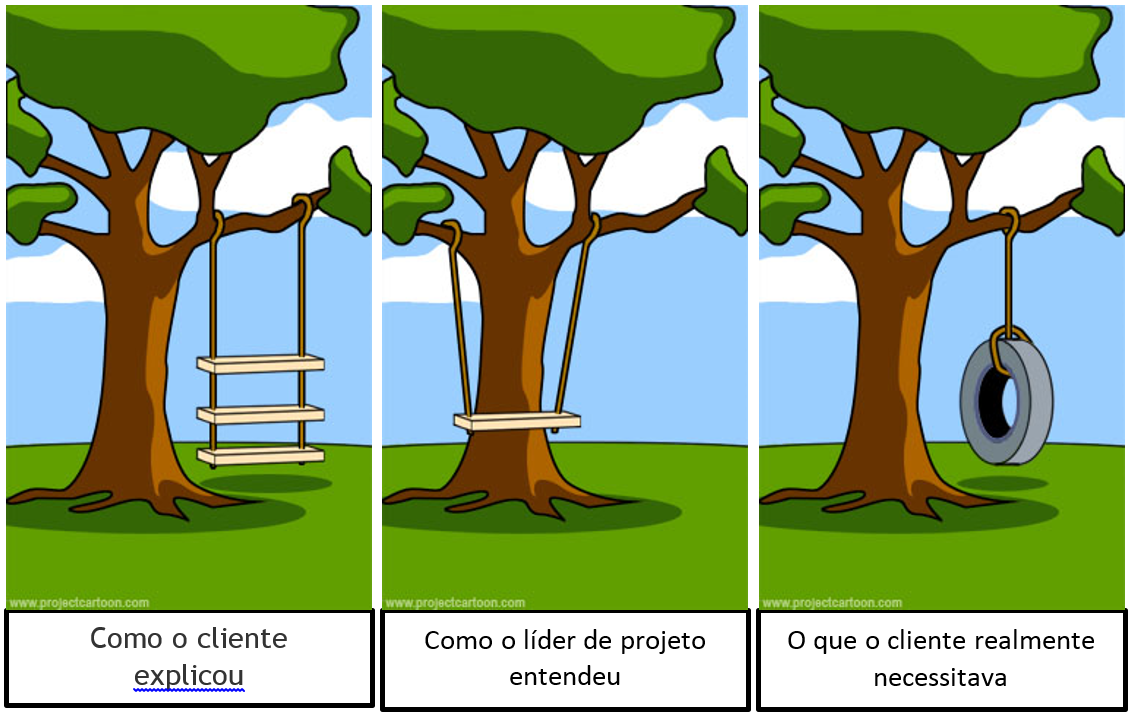
\includegraphics[width=0.90\textwidth]{figuras/The-Project-Cartoon-Beta.png}
    \caption{A importância do Levantamento de Requisitos}
    \label{fig:levantamento:requisitos}
\end{figure}

%---------------------------------------------------%
\section{Exemplo de uso de Equação}
\label{cap:conceitos:sec:usando:equacoes}

O valor mensurado do tráfego de bytes considerando todos os níveis da hierarquia de memória ($Q_{total}$) é calculado usando a Equação \ref{equ:roofline:qtotal}.

\begin{equation}\label{equ:roofline:qtotal}
Q_{total} = Q_{L1} + Q_{L2} + Q_{LLC} + Q_{MEM}
\end{equation}

%---------------------------------------------------%
\section{Usando Código}
\label{cap:conceitos:sec:usando:codigo}

Se for necessário apresentar a ideia de um Algoritmo~\ref{alg:decisao-001} em pseudocódigo...

\begin{algorithm}[H]
	\caption{Meu algoritmo}
	\label{alg:decisao-001}
	\begin{algorithmic}[1]
		\STATE $\textbf{INPUT:}*better\_device\_index$
		\STATE $\textbf{OUTPUT:} *better\_device\_index, offload\_decison$
		\STATE $offload\_decision \leftarrow true$
		\IF{($offload\_decision \leftarrow \textbf{RM\_check\_all\_eventsets\_was\_collected(})$)}
		\STATE $oi \leftarrow \textbf{RM\_get\_operational\_intensity}()$
		\STATE $better\_device\_index \leftarrow \textbf{RM\_get\_better\_device\_to\_execution}(oi)$ 
		\ELSE
		\STATE {$better\_device\_index \leftarrow 0$}	
		\ENDIF
		\RETURN $offload\_decision$
	\end{algorithmic}
\end{algorithm}

O Código~\ref{cod:omp:directive:parallel} apresenta um código colocado diretamente no texto e usando a opção \textit{language} que utilizará as definições de formatação para a linguagem...

\begin{lstlisting}[language=C, basicstyle=\small, label=cod:omp:directive:parallel, caption={Parallel directive format}]
#pragma omp parallel
{
	body;
}
\end{lstlisting}

Com o pacote \texttt{listings} pode também ser utilizado com um estilo usando a opção \textit{style}. Veja as definições no arquivo de configurações. O Código~\ref{cod:hello:world} apresenta um código na linguagem \texttt{C} aplicando um estilo.

\begin{lstlisting}[style=C, label=cod:hello:world, caption={Hello World Estilizado}]
#include <stdio.h>
int main(){
  printf("Hello World!!!");
  return 0;
}
\end{lstlisting}

Código~\ref{cod:incluido:do:dir:src} mostra como incluir um código de um diretório \texttt{src} caso opte por utilizar assim... É possível escolher um intervalo de linhas para serem apresentadas com a opção \texttt{linerange}.

\lstinputlisting[style=C, label=cod:incluido:do:dir:src,caption=Código da pasta \texttt{src}, linerange={48-51},firstnumber=1]{src/exemplo.c}


%---------------------------------------------------%
\section{Usando Tabelas}
\label{cap:conceitos:sec:usando:tabelas}

Na Tabela~\ref{tab:exemplo-001} são listados/apresentados...

\begin{table}[h!]
\renewcommand{\arraystretch}{1.3}
\caption{Legenda de Tabela é em cima}
\label{tab:exemplo-001}
\centering
\begin{tabular}{|@{$~$}l@{ }||@{$~$}l@{ }|@{$~$}l@{ }|}
\hline
\textbf{Coluna 1} & \textbf{Coluna 2} & \textbf{Coluna 3} \\
\hline
\begin{minipage}[t]{0.10\textwidth}%
\texttt{Bla Bla} %
\end{minipage} & 
\begin{minipage}[t]{0.30\textwidth}%
  TEXTO TEXTO TEXTO TEXTO TEXTO TEXTO TEXTO TEXTO TEXTO TEXTO TEXTO TEXTO TEXTO TEXTO TEXTO TEXTO TEXTO TEXTO TEXTO TEXTO TEXTO TEXTO TEXTO TEXTO TEXTO TEXTO TEXTO TEXTO TEXTO TEXTO TEXTO TEXTO TEXTO %
\end{minipage} &
\begin{minipage}[t]{0.50\textwidth}%
TEXTO TEXTO TEXTO TEXTO TEXTO TEXTO TEXTO TEXTO TEXTO TEXTO TEXTO TEXTO TEXTO TEXTO TEXTO TEXTO TEXTO TEXTO TEXTO TEXTO TEXTO TEXTO TEXTO TEXTO TEXTO TEXTO TEXTO TEXTO TEXTO TEXTO TEXTO TEXTO TEXTO TEXTO TEXTO TEXTO TEXTO TEXTO TEXTO TEXTO TEXTO TEXTO TEXTO TEXTO TEXTO TEXTO TEXTO TEXTO TEXTO TEXTO TEXTO TEXTO TEXTO TEXTO TEXTO TEXTO TEXTO TEXTO TEXTO TEXTO TEXTO TEXTO TEXTO TEXTO TEXTO TEXTO%
\end{minipage}
\tabularnewline
\hline
\begin{minipage}[t]{0.10\textwidth}%
Bla Bla 2 %
\end{minipage} & 
\begin{minipage}[t]{0.30\textwidth}%
TEXTO TEXTO TEXTO TEXTO TEXTO TEXTO TEXTO TEXTO TEXTO TEXTO TEXTO TEXTO TEXTO TEXTO TEXTO TEXTO TEXTO TEXTO TEXTO TEXTO TEXTO TEXTO TEXTO TEXTO TEXTO TEXTO TEXTO TEXTO TEXTO TEXTO TEXTO TEXTO TEXTO %
\end{minipage} &
\begin{minipage}[t]{0.50\textwidth}%
TEXTO TEXTO TEXTO TEXTO TEXTO TEXTO TEXTO TEXTO TEXTO TEXTO TEXTO TEXTO TEXTO TEXTO TEXTO TEXTO TEXTO TEXTO TEXTO TEXTO TEXTO TEXTO %
\end{minipage}
\tabularnewline
\hline
\end{tabular}
\end{table}

%---------------------------------------------------%
\section{Considerações Finais}
\label{cap:conceitos:sec:consideracoes:finais}

Esta é uma sugestão de seção para dar um fechamento em cada uma dos capítulos.

(ATENÇÃO - veja com o seu orientador se é uma seção necessária (pois trate-se de estilo de escrita))